\documentclass[tikz,border=10pt]{standalone}
\usepackage{amsmath}
\usepackage{amssymb}
\usepackage{tikz}
\usetikzlibrary{arrows.meta,calc}

\definecolor{figazul}{RGB}{2,132,199}
\definecolor{figrojo}{RGB}{220,38,38}
\definecolor{figverde}{RGB}{22,163,74}

\begin{document}
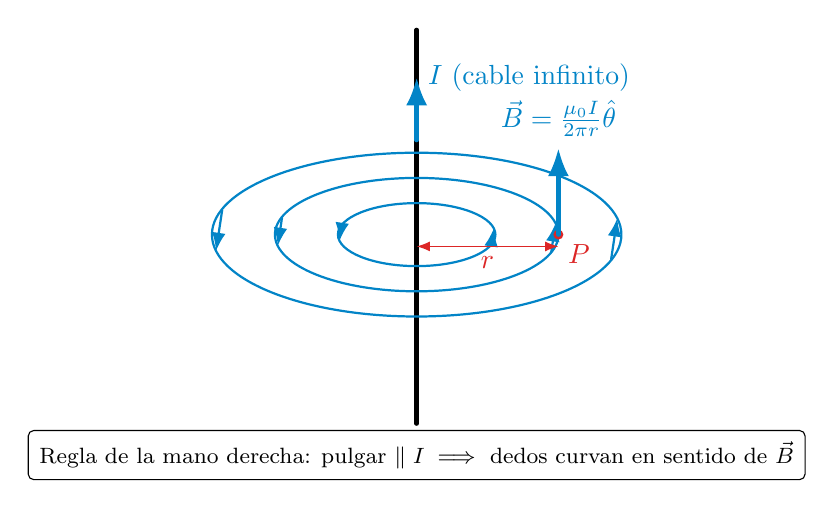
\begin{tikzpicture}[>=Latex, line cap=round, line join=round]
  % Cable infinito vertical a lo largo de z
  \draw[ultra thick, color=black] (0, -2.4) -- (0, 2.6);
  \draw[->, ultra thick, color=figazul] (0, 1.2) -- (0, 2.0) node[right, color=figazul] {$I$ (cable infinito)};

  % Líneas de campo magnético circulares concéntricas en perspectiva (elipses)
  % Nivel z = 0
  \foreach \r in {1.0, 1.8, 2.6} {
    \draw[thick, color=figazul] (0,0) ellipse ({\r} and {\r*0.4});
    % Flechas de circulación azimutal (regla de la mano derecha: antihorario visto desde arriba)
    \draw[->, thick, color=figazul] ({\r*0.95}, {-\r*0.4*0.3}) -- ({\r*0.98}, {\r*0.4*0.2});
    \draw[->, thick, color=figazul] ({-\r*0.95}, {\r*0.4*0.3}) -- ({-\r*0.98}, {-\r*0.4*0.2});
  }

  % Vector B en un punto de observación a distancia r
  \coordinate (P) at (1.8, 0);
  \fill[color=figrojo] (P) circle (1.8pt) node[below right, color=figrojo] {$P$};
  \draw[<->, thin, color=figrojo] (0, -0.15) -- (1.8, -0.15) node[midway, below, color=figrojo] {$r$};
  \draw[->, ultra thick, color=figazul] (P) -- ($(P) + (0, 1.1)$) node[above, color=figazul] {$\vec{B} = \frac{\mu_0 I}{2\pi r}\hat{\theta}$};

  % Indicación de regla mano derecha
  \node[draw, rounded corners=2pt, inner sep=4pt, fill=white, fill opacity=0.9, text opacity=1, font=\footnotesize] at (0, -2.8)
    {Regla de la mano derecha: pulgar $\parallel I \implies$ dedos curvan en sentido de $\vec{B}$};
\end{tikzpicture}
\end{document}
